\documentclass[12pt,a4paper]{article}

\usepackage[utf8]{vietnam}
\usepackage{geometry}
\usepackage{graphicx}
\usepackage{amsmath}
\usepackage{amssymb}
\usepackage{float}
\usepackage{booktabs}
\usepackage{longtable}
\usepackage{array}
\usepackage{xcolor}
\usepackage{listings}
\usepackage{enumitem}
\usepackage{hyperref}
\usepackage{caption}
\usepackage{subcaption}

\geometry{left=2.8cm,right=2.2cm,top=2.5cm,bottom=2.5cm}
\hypersetup{
    colorlinks=true,
    linkcolor=blue,
    urlcolor=blue,
    citecolor=blue
}
\setlength{\parindent}{0pt}
\setlength{\parskip}{6pt}
\renewcommand{\arraystretch}{1.2}
\newcolumntype{P}[1]{>{\raggedright\arraybackslash}p{#1}}

\lstset{
    basicstyle=\ttfamily\small,
    breaklines=true,
    frame=single,
    columns=fullflexible,
    backgroundcolor=\color{gray!8}
}

\title{\textbf{BÁO CÁO ĐỒ ÁN}\\[0.4cm]
\Large Hệ thống định danh người dùng qua hành vi sử dụng điện thoại}
\author{
Môn học: Nhập môn Khoa học dữ liệu\\
Nhóm thực hiện: Nhóm đồ án NMKHDL
}
\date{Ngày biên soạn: 24/05/2026}

\begin{document}

\hypersetup{pageanchor=false}
\begin{titlepage}
    \centering
    {\Large \textbf{ĐẠI HỌC BÁCH KHOA HÀ NỘI}}\\
    {\large Trường Công nghệ Thông tin và Truyền thông}\\[2.0cm]

    {\LARGE \textbf{BÁO CÁO ĐỒ ÁN}}\\[0.6cm]
    {\Large \textbf{Hệ thống định danh người dùng qua hành vi sử dụng điện thoại}}\\[1.2cm]

    \begin{tabular}{rl}
        Môn học: & Nhập môn Khoa học dữ liệu \\
        Hướng tiếp cận: & Random Forest, SVM (RBF) và CNN 1D \\
        Dữ liệu: & Hành vi cảm biến điện thoại và gõ phím \\
    \end{tabular}\\[1.6cm]

    \textbf{Thành viên nhóm}\\[0.3cm]
    \begin{tabular}{ll}
        Lương Mạnh Tường & 20225949 \\
        Bùi Minh Tuấn & 20225678 \\
        Trương Quốc Triệu & 20225941 \\
        Nguyễn Đức Thành & 20225930 \\
        Nguyễn Anh Tuấn & 20225772 \\
        Vũ Ngọc Lâm & 20225645 \\
        Vũ Nhật Quang & 20225761 \\
        Mai Văn Đăng & 20225699 \\
        Nguyễn Đình Thành & 20225670 \\
    \end{tabular}

    \vfill
    Hà Nội, 05/2026
\end{titlepage}

\hypersetup{pageanchor=true}
\pagenumbering{roman}
\tableofcontents
\newpage
\pagenumbering{arabic}

\section*{Tóm tắt}
\addcontentsline{toc}{section}{Tóm tắt}

Đồ án khảo sát bài toán định danh người dùng từ dữ liệu sử dụng điện thoại theo chế độ closed-set với 15 người dùng. Phần mô hình chính dùng tín hiệu cảm biến quán tính; log gõ phím được giữ như nguồn dữ liệu phụ để kiểm tra và mở rộng sau. Ba mô hình được so sánh: Random Forest và SVM (RBF) trên 65 đặc trưng thủ công, cùng CNN 1D học trực tiếp trên chuỗi cảm biến. Với cách đánh giá 3-fold \textit{StratifiedGroupKFold} chia theo file để tránh rò rỉ dữ liệu, Random Forest đạt macro-F1 trung bình 0.7434, SVM (RBF) đạt 0.6550, và CNN 1D simple đạt 0.6272. Trên tập dữ liệu hiện tại với số phiên ghi giới hạn cho mỗi người dùng, hai mô hình dùng đặc trưng thống kê thủ công cho macro-F1 cao hơn CNN 1D học đặc trưng tự động.

\newpage

\section{Mô tả bài toán thực tế}

\subsection{Bối cảnh}

Điện thoại cá nhân thường chứa tài khoản, tin nhắn, ảnh và nhiều dữ liệu nhạy cảm. Mật khẩu, vân tay hoặc nhận diện khuôn mặt bảo vệ tốt ở thời điểm mở khoá, nhưng không theo dõi liên tục trong quá trình sử dụng. Sinh trắc học hành vi tiếp cận vấn đề từ một góc khác: nhận ra người dùng qua cách họ cầm, di chuyển và thao tác với thiết bị.

Trong đồ án này, hệ thống cần dự đoán người đang sử dụng điện thoại từ dữ liệu hành vi. Nguồn chính là chuyển động của điện thoại khi người dùng ngồi, đứng và đi bộ; dữ liệu gõ phím được dùng để ghi nhận thêm nhịp tương tác.

\subsection{Phát biểu bài toán}

Với mỗi mẫu dữ liệu cảm biến quán tính có dạng chuỗi thời gian:
\[
X_i \in \mathbb{R}^{128 \times 6}
\]
trong đó 128 là số mẫu trong một cửa sổ 2.56 giây, 6 kênh gồm \texttt{acc\_x, acc\_y, acc\_z, gyro\_x, gyro\_y, gyro\_z}. Mục tiêu là học hàm phân loại:
\[
f(X_i) \rightarrow y_i, \quad y_i \in \{1, 2, \dots, 15\}
\]
với \(y_i\) là mã của một trong 15 người dùng trong dữ liệu.

Đồ án giải bài toán ở chế độ \textbf{closed-set}: mọi mẫu kiểm thử đều thuộc về một trong 15 người dùng đã xuất hiện trong huấn luyện. Phạm vi closed-set cho phép tập trung đánh giá khả năng phân biệt người dùng giữa các mô hình trên cùng một tập lớp cố định. Bài toán phát hiện người dùng lạ (open-set) nằm ngoài phạm vi đồ án vì đòi hỏi thêm dữ liệu người dùng chưa biết và phương pháp ước lượng ngưỡng riêng.

\subsection{Ý nghĩa thực tế}

Nếu đạt độ tin cậy đủ cao, hướng này có thể dùng cho xác thực liên tục hoặc cảnh báo khi thiết bị có dấu hiệu bị người khác sử dụng. Trong đồ án, trọng tâm là xây dựng pipeline dữ liệu có thể chạy lại, chia train/validation đúng cách và giải thích rõ giới hạn của kết quả.

\section{Phương pháp học máy và dataset sử dụng}

\subsection{Dataset}

Bộ dữ liệu dùng trong báo cáo gồm 15 người dùng và 185 file CSV sau khi bỏ các log không dùng trong pipeline cuối. Các file còn lại được chia thành hai nhóm:

\begin{itemize}
    \item \textbf{Inertial}: dữ liệu cảm biến quán tính, gồm gia tốc kế và con quay hồi chuyển. Đây là nguồn dữ liệu chính dùng cho mô hình.
    \item \textbf{Keystroke}: dữ liệu gõ phím như thời điểm gõ, khoảng cách thời gian giữa các phím, tốc độ gõ.
\end{itemize}

Sau bước quét dữ liệu, \texttt{manifest.csv} được sinh ra để chuẩn hoá thông tin: người dùng, tên file, modality, hoạt động, session, attempt/rep, số dòng và tần số lấy mẫu ước lượng. Bảng \ref{tab:modality-counts} và \ref{tab:activity-counts} tóm tắt quy mô dữ liệu sau khi chuẩn hoá manifest.

\begin{table}[H]
    \centering
    \caption{Số lượng file theo modality}
    \label{tab:modality-counts}
    \begin{tabular}{lc}
        \toprule
        Modality & Số file \\
        \midrule
        Inertial & 154 \\
        Keystroke & 31 \\
        \midrule
        Tổng & 185 \\
        \bottomrule
    \end{tabular}
\end{table}

\begin{table}[H]
    \centering
    \caption{Số file inertial theo hoạt động}
    \label{tab:activity-counts}
    \begin{tabular}{lc}
        \toprule
        Hoạt động & Số file inertial \\
        \midrule
        sitting & 46 \\
        standing & 46 \\
        walking & 62 \\
        \bottomrule
    \end{tabular}
\end{table}

Mô hình chính dùng inertial vì đây là chuỗi thời gian liên tục và khớp trực tiếp với cả hai hướng mô hình: Random Forest trên đặc trưng thống kê và CNN 1D trên tín hiệu thô đã xử lý. Keystroke được trích đặc trưng trong \texttt{features.py} nhưng chưa đưa vào kết quả chính, để phần đánh giá tập trung vào một nguồn tín hiệu rõ ràng. Tần số lấy mẫu thực tế giữa các file không hoàn toàn đồng nhất, vì vậy pipeline có bước resample về 50 Hz trước khi chia cửa sổ.

\subsection{Tiền xử lý dữ liệu cảm biến}

Pipeline tiền xử lý được cài đặt trong \texttt{preprocess.py}. Các bước chính:

\begin{enumerate}
    \item Đọc dữ liệu cảm biến từ CSV.
    \item Điền giá trị thiếu bằng forward-fill/backward-fill.
    \item Resample về 50 Hz nếu tần số lấy mẫu thực tế lệch nhiều.
    \item Lọc low-pass Butterworth cutoff 20 Hz để giảm nhiễu cao tần.
    \item Lọc high-pass Butterworth cutoff 0.3 Hz cho ba trục gia tốc để tách thành phần trọng lực.
    \item Chia cửa sổ 128 mẫu, bước trượt 64 mẫu, tương đương overlap 50\%.
    \item Giới hạn tối đa 300 cửa sổ mỗi file để tránh một file dài chi phối toàn bộ tập huấn luyện.
\end{enumerate}

Kết quả lưu tại \texttt{windows.npz} với tensor:

\[
X \in \mathbb{R}^{39018 \times 128 \times 6}
\]

Hình \ref{fig:preprocess} minh hoạ tác dụng của bước lọc tín hiệu trên một đoạn dữ liệu walking của \texttt{userA}. Tín hiệu thô (đường xám) chứa nhiễu cao tần và thành phần trọng lực một chiều; sau khi lọc low-pass 20 Hz và high-pass 0.3 Hz, tín hiệu (đường màu) mượt hơn và dao động quanh gốc do thành phần trọng lực đã bị tách khỏi ba trục gia tốc.

\begin{figure}[H]
    \centering
    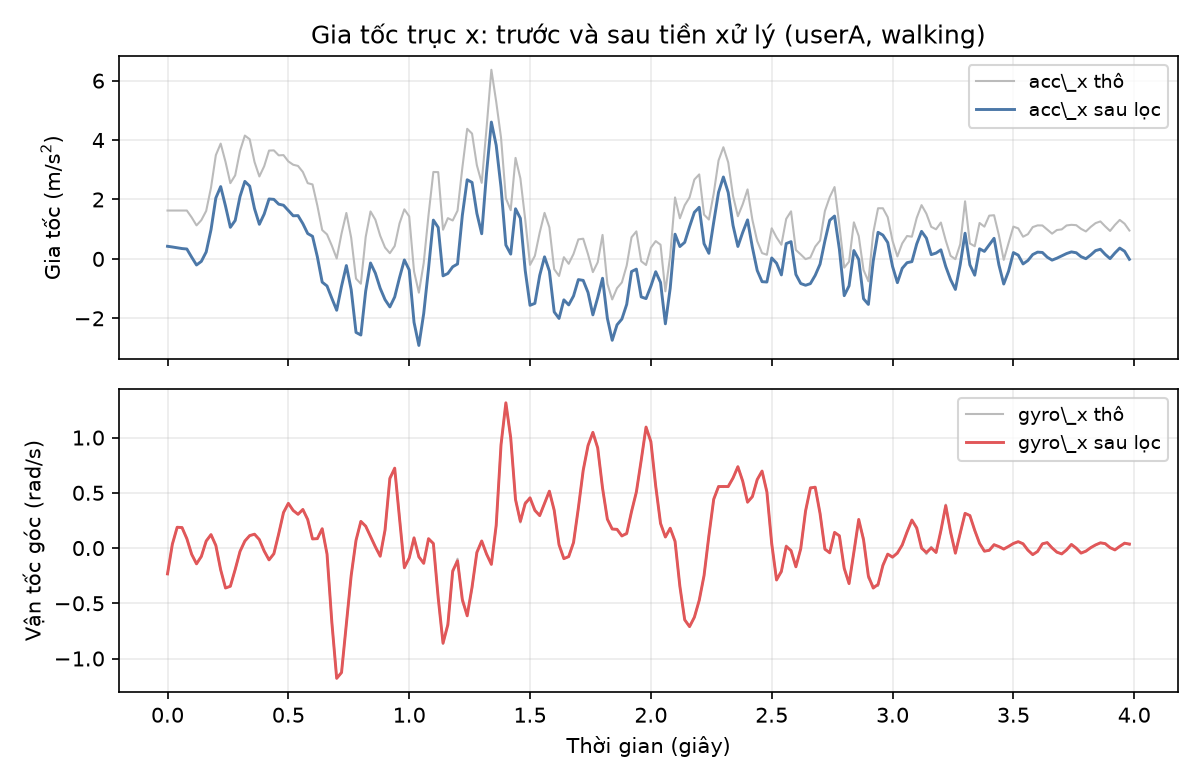
\includegraphics[width=0.92\textwidth]{figures/preprocess_raw_vs_filtered.png}
    \caption{Tín hiệu gia tốc và vận tốc góc trước (xám) và sau (màu) bước tiền xử lý lọc Butterworth}
    \label{fig:preprocess}
\end{figure}

Hình \ref{fig:window} minh hoạ cách chia cửa sổ trượt: mỗi cửa sổ dài 128 mẫu (2.56 giây) và bước trượt 64 mẫu, nên hai cửa sổ liên tiếp chồng lấn 50\%. Cách này giữ tính liên tục của tín hiệu giữa các cửa sổ và tăng số mẫu huấn luyện, nhưng đồng thời tạo ra các cửa sổ gần giống nhau trong cùng một file, là lý do cần chia dữ liệu theo file ở phần sau.

\begin{figure}[H]
    \centering
    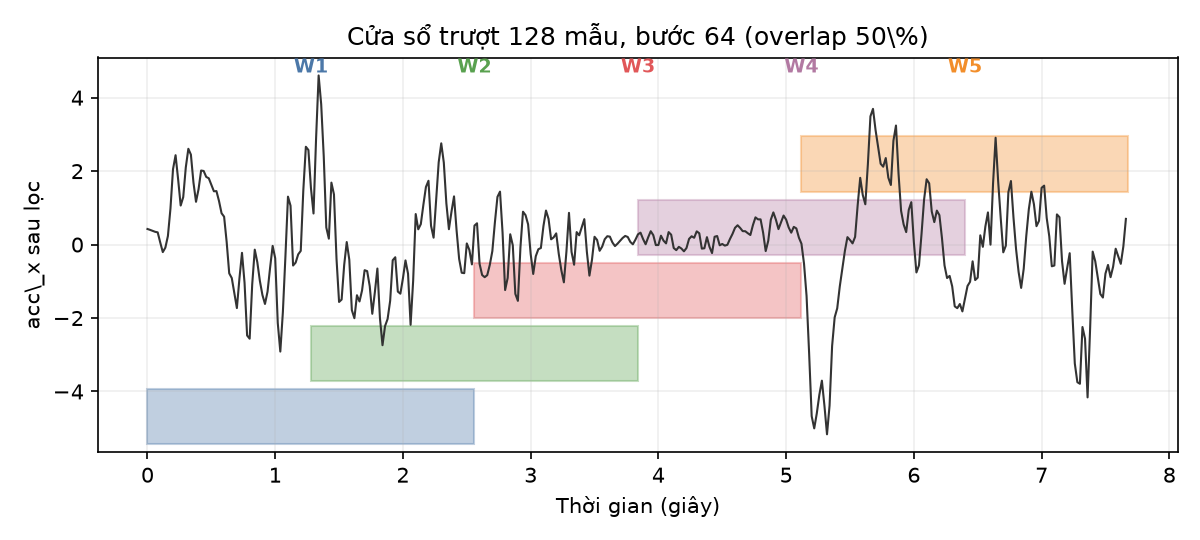
\includegraphics[width=0.92\textwidth]{figures/window_segmentation.png}
    \caption{Cửa sổ trượt 128 mẫu với bước 64 (overlap 50\%) trên tín hiệu đã lọc}
    \label{fig:window}
\end{figure}

\subsection{Cách chia dữ liệu}

Sau tiền xử lý, tập inertial có 39018 cửa sổ, mỗi cửa sổ có kích thước \((128, 6)\). 15 người dùng trong dữ liệu gồm \texttt{userA}, \texttt{userB}, \texttt{userC}, \texttt{userD}, \texttt{userE}, \texttt{userF}, \texttt{userG}, \texttt{userH}, \texttt{userI}, \texttt{userK}, \texttt{userL}, \texttt{userM}, \texttt{userN}, \texttt{userP}, \texttt{userQ}. Vì là bài toán closed-set, cả 15 người dùng đều tham gia huấn luyện và đánh giá; việc chia dữ liệu được thực hiện ở mức file để phục vụ cross-validation.

\begin{table}[H]
    \centering
    \caption{Quy mô dữ liệu closed-set 15 người dùng}
    \label{tab:closed-set}
    \begin{tabular}{lccc}
        \toprule
        Tập & Users & Windows & Groups/files \\
        \midrule
        Closed-set & 15 & 39018 & 154 \\
        \bottomrule
    \end{tabular}
\end{table}

Với toàn bộ 15 người dùng, nhóm dùng \textit{StratifiedGroupKFold}. Điểm quan trọng là \textbf{không chia ngẫu nhiên theo cửa sổ}. Vì sliding window tạo ra nhiều cửa sổ liên tiếp, các cửa sổ gần nhau trong cùng một file có nội dung tín hiệu rất giống nhau. Nếu random split theo cửa sổ, train và validation có thể cùng chứa các đoạn gần như trùng từ một phiên ghi, làm mô hình học đặc trưng của phiên ghi thay vì học hành vi người dùng. Đây là dạng data leakage và thường làm điểm đánh giá cao giả tạo.

Để tránh leakage, mỗi cửa sổ được gắn group có dạng \texttt{user\_\_file}. Khi chia fold, toàn bộ cửa sổ sinh ra từ cùng một file luôn nằm trọn trong train hoặc trọn trong validation. Như vậy validation mô phỏng một phiên ghi mới hơn, khó hơn và gần thực tế hơn so với random split theo cửa sổ. Thành phần \textit{stratified} giúp phân phối user trong các fold tương đối cân bằng, còn \textit{group} đảm bảo ràng buộc không tách cùng một file sang hai tập. Tham số \texttt{shuffle=True, random\_state=42} được dùng để kết quả có thể tái lập.

Nhóm chọn 3-fold vì số file giữa các user không đều; user ít file nhất là \texttt{userQ}, chỉ có 3 file inertial. Nếu dùng 5-fold, một số fold validation có nguy cơ thiếu class, khiến macro-F1 không còn phản ánh đủ 15 người dùng. Với 3-fold, mỗi fold vẫn có đủ lớp để đánh giá ổn định hơn.

\begin{table}[H]
    \centering
    \caption{Thống kê train/validation của 3 fold closed-set}
    \label{tab:fold-split-stats}
    \begin{tabular}{lrrrr}
        \toprule
        Fold & Train windows & Val windows & Train groups & Val groups \\
        \midrule
        1 & 26207 & 12811 & 102 & 52 \\
        2 & 25585 & 13433 & 103 & 51 \\
        3 & 26244 & 12774 & 103 & 51 \\
        \bottomrule
    \end{tabular}
\end{table}

Hình \ref{fig:split} minh hoạ nguyên tắc chia: mỗi ô là một cửa sổ, các ô cùng màu thuộc cùng một fold, và ranh giới trắng phân tách các file. Toàn bộ cửa sổ sinh ra từ một file luôn nằm trọn trong một fold, nên không có cửa sổ nào của cùng một phiên ghi bị tách sang cả train lẫn validation.

\begin{figure}[H]
    \centering
    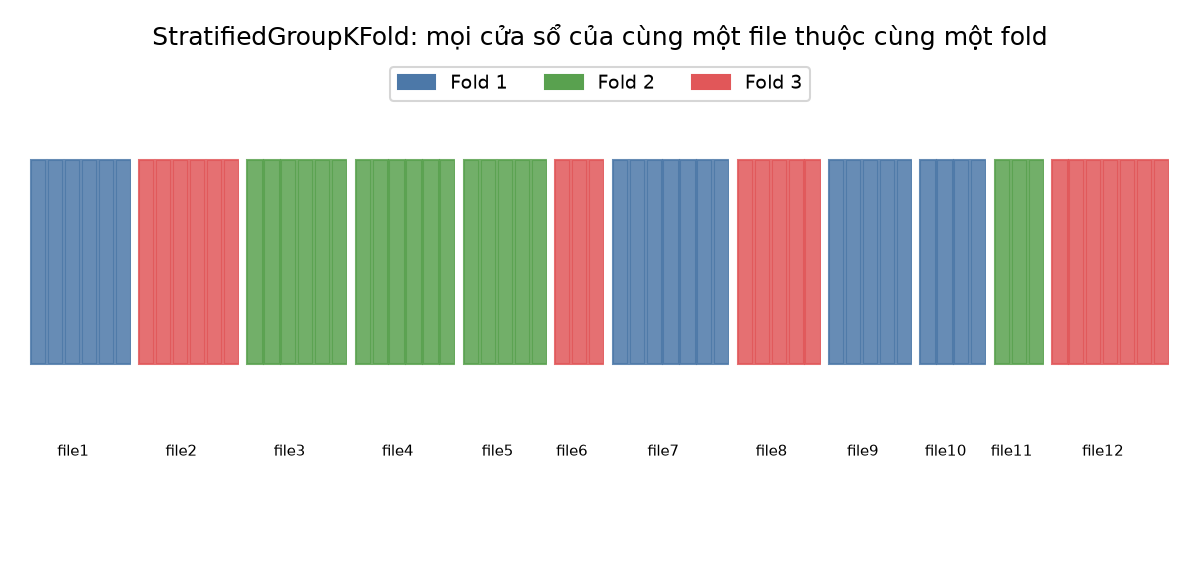
\includegraphics[width=0.92\textwidth]{figures/split_scheme.png}
    \caption{Nguyên tắc StratifiedGroupKFold: các cửa sổ của cùng một file (group) luôn thuộc cùng một fold}
    \label{fig:split}
\end{figure}

\subsection{Mô hình Random Forest}

Random Forest là mô hình ensemble gồm nhiều cây quyết định, phù hợp với dữ liệu dạng bảng có số chiều vừa phải. Mỗi cửa sổ cảm biến được chuyển thành vector 65 đặc trưng thủ công. Cấu trúc feature gồm \(6 \times 9 = 54\) đặc trưng thống kê/FFT cho 6 kênh, 9 đặc trưng correlation giữa các cặp trục được chọn, và 2 đặc trưng Signal Magnitude Area (SMA) cho accelerometer và gyroscope.

\begin{itemize}
    \item Thống kê theo từng trục: mean, standard deviation, MAD, min, max, IQR, energy.
    \item Đặc trưng miền tần số: FFT entropy, dominant frequency.
    \item Tương quan giữa các trục.
    \item Signal Magnitude Area cho accelerometer và gyroscope.
\end{itemize}

Mô hình sử dụng \texttt{RandomForestClassifier} với 300 cây. Tham số cân bằng lớp là \texttt{class\_weight=balanced\_subsample}. Random Forest không yêu cầu chuẩn hoá đặc trưng và ít nhạy với khác biệt thang đo giữa các đặc trưng thống kê; cơ chế bagging trên 300 cây giảm phương sai dự đoán khi số mẫu mỗi người dùng không đều. Tham số \texttt{class\_weight=balanced\_subsample} tính lại trọng số lớp trên từng mẫu bootstrap, bù cho mất cân bằng số cửa sổ giữa các người dùng.

Để tránh leakage ở bước chuẩn hoá, \texttt{StandardScaler} chỉ được fit trên train fold. Sau đó scaler này mới được dùng để transform validation fold. Quy trình này đảm bảo validation không tham gia vào việc ước lượng trung bình và độ lệch chuẩn của đặc trưng.

\subsection{Mô hình SVM (RBF)}

SVM với kernel RBF được thêm như mô hình thứ ba, dùng \textbf{đúng 65 đặc trưng thủ công} như Random Forest. Lý do chọn SVM RBF là để bổ sung một góc nhìn khác về bản chất: trong khi Random Forest là mô hình dạng cây chia không gian theo các ngưỡng trục, SVM RBF là mô hình \textit{margin-based} tìm siêu phẳng phân tách với biên lớn nhất trong không gian đặc trưng được ánh xạ phi tuyến. So sánh hai mô hình cùng đầu vào nhưng khác nguyên lý giúp kiểm chứng xem kết quả tốt đến từ chất lượng đặc trưng hay từ một loại mô hình cụ thể.

Cấu hình: \texttt{SVC(kernel="rbf", C=10, gamma="scale", class\_weight="balanced")}.

\begin{itemize}
    \item \textbf{Kernel RBF}: cho phép tạo biên quyết định phi tuyến, phù hợp khi ranh giới giữa các người dùng trong không gian 65 chiều không tuyến tính.
    \item \(\mathbf{C=10}\): tham số phạt lỗi; giá trị vừa phải này ưu tiên phân loại đúng tập huấn luyện hơn mức mặc định \(C=1\) nhưng vẫn giữ regularization để tránh overfit.
    \item \texttt{gamma="scale"}: tự co giãn theo phương sai đặc trưng, tránh phải dò tay.
    \item \texttt{class\_weight="balanced"}: bù cho việc số cửa sổ giữa các người dùng không đều, tương tự \texttt{balanced\_subsample} của Random Forest.
\end{itemize}

Khác với Random Forest, SVM RBF \textbf{bắt buộc} chuẩn hoá đặc trưng vì kernel RBF tính khoảng cách Euclid giữa các mẫu; nếu một đặc trưng có thang đo lớn (ví dụ energy) sẽ lấn át các đặc trưng nhỏ. Vì vậy \texttt{StandardScaler} cũng chỉ fit trên train fold rồi áp lên validation, giống quy trình của Random Forest để so sánh công bằng.

\subsection{Mô hình CNN 1D}

CNN 1D được dùng để kiểm tra khả năng học trực tiếp từ chuỗi cảm biến. Sau khi đi qua \texttt{InertialDataset}, dữ liệu đầu vào có dạng \((B, 6, 128)\), trong đó \(B\) là batch size, 6 là số kênh cảm biến, 128 là chiều thời gian. Conv1D trượt kernel theo trục thời gian để học các mẫu biến thiên ngắn hạn của accelerometer và gyroscope.

\begin{lstlisting}
Input: (6, 128)
Conv1D(6 -> 32, kernel=7) + BatchNorm + ReLU + MaxPool
Conv1D(32 -> 64, kernel=5) + BatchNorm + ReLU + MaxPool
Conv1D(64 -> 128, kernel=3) + BatchNorm + ReLU
AdaptiveAvgPool1D
Dropout(0.3)
Linear(128 -> 15)
\end{lstlisting}

Trong kiến trúc này, BatchNorm giúp ổn định phân phối activation trong quá trình huấn luyện; ReLU tạo phi tuyến; MaxPool giảm chiều thời gian và giữ mẫu nổi bật; AdaptiveAvgPool gom toàn bộ chuỗi thành một vector cố định trước khi phân loại; Dropout giảm overfit. Kiến trúc được giới hạn ở 3 tầng convolution để số tham số tương xứng với quy mô dữ liệu (39018 cửa sổ), tránh overfit khi mô hình quá lớn so với lượng mẫu huấn luyện.

Cấu hình huấn luyện:

\begin{itemize}
    \item Optimizer: Adam.
    \item Learning rate: 0.001.
    \item Loss: CrossEntropy có class weight nghịch tần suất.
    \item Epoch: 40.
    \item Batch size: 128.
    \item Không dùng scheduler, không dùng MixUp/CutMix, không dùng sweep nhiều phase.
\end{itemize}

Cấu hình không dùng scheduler hay augmentation nhằm cô lập đóng góp của kiến trúc CNN cơ sở: kết quả phản ánh năng lực của mô hình base mà không bị ảnh hưởng bởi các kỹ thuật tăng cường, giúp so sánh trực tiếp với hai mô hình cổ điển trên cùng điều kiện huấn luyện tối giản.

\section{Kết quả thí nghiệm đánh giá hiệu năng}

\subsection{Chỉ số đánh giá}

Nhóm sử dụng nhiều chỉ số vì mỗi chỉ số phản ánh một khía cạnh khác nhau của hệ thống:

\begin{itemize}
    \item \textbf{Accuracy}: tỷ lệ dự đoán đúng trên toàn bộ mẫu. Khi số cửa sổ giữa các người dùng không đều, accuracy bị chi phối bởi các lớp có nhiều mẫu hơn.
    \item \textbf{Macro-F1}: tính F1 riêng cho từng người dùng rồi lấy trung bình không trọng số. Mỗi người dùng đóng góp ngang nhau vào điểm cuối, nên một người dùng ít dữ liệu bị dự đoán sai sẽ kéo điểm xuống rõ rệt. Do tập dữ liệu mất cân bằng giữa các lớp, macro-F1 được dùng làm chỉ số chính để xếp hạng mô hình.
\end{itemize}

Với \(C\) class người dùng, macro-F1 được tính theo:

\[
MacroF1 = \frac{1}{C}\sum_{c=1}^{C} F1_c
\]

\subsection{Kết quả tổng thể}

Kết quả được chạy lại với cấu hình đơn giản, lưu tại \texttt{simple\_results.json}. Bảng \ref{tab:main-results} trình bày điểm trung bình trên 3 fold.

\begin{table}[H]
    \centering
    \caption{Kết quả closed-set theo 3-fold StratifiedGroupKFold}
    \label{tab:main-results}
    \begin{tabular}{lccc}
        \toprule
        Mô hình & Macro-F1 trung bình & Độ lệch chuẩn & Accuracy trung bình \\
        \midrule
        CNN 1D simple & 0.6272 & 0.0336 & 0.6523 \\
        Random Forest & \textbf{0.7434} & 0.0517 & \textbf{0.7482} \\
        SVM (RBF) & 0.6550 & 0.0456 & 0.6740 \\
        \bottomrule
    \end{tabular}
\end{table}

\begin{figure}[H]
    \centering
    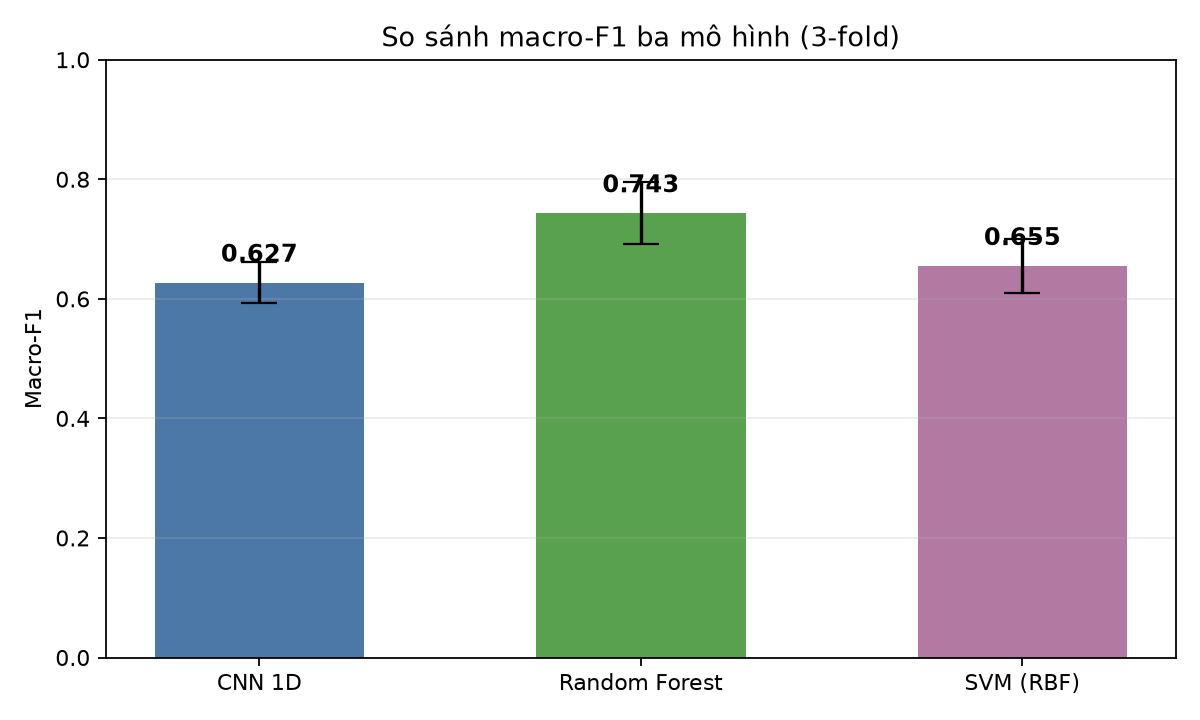
\includegraphics[width=0.78\textwidth]{figures/simple_model_comparison.png}
    \caption{So sánh macro-F1 giữa CNN 1D, Random Forest và SVM (RBF)}
    \label{fig:model-comparison}
\end{figure}

Từ kết quả ở Bảng \ref{tab:main-results}, có thể thấy mô hình Random Forest đạt hiệu năng vượt trội nhất với Macro-F1 trung bình là 0.7434 và Accuracy trung bình là 0.7482. SVM (RBF) đứng thứ hai với Macro-F1 trung bình 0.6550. Trong khi đó, mô hình học sâu CNN 1D đạt kết quả thấp nhất với Macro-F1 trung bình là 0.6272. Sự vượt trội của Random Forest so với CNN 1D cho thấy đối với tập dữ liệu có kích thước vừa phải và số lượng phiên ghi của mỗi người dùng còn hạn chế, các đặc trưng thống kê được thiết kế thủ công (hand-crafted features) vẫn mang lại độ chính xác và độ ổn định cao hơn so với việc để mô hình deep learning tự học các biểu diễn từ chuỗi tín hiệu thô.

\subsection{Độ ổn định theo fold}

\begin{table}[H]
    \centering
    \caption{Macro-F1 trên từng fold}
    \label{tab:fold-results}
    \begin{tabular}{lccc}
        \toprule
        Mô hình & Fold 1 & Fold 2 & Fold 3 \\
        \midrule
        CNN 1D simple & 0.6578 & 0.5804 & 0.6436 \\
        Random Forest & 0.7607 & 0.6732 & 0.7962 \\
        SVM (RBF) & 0.6660 & 0.5944 & 0.7046 \\
        \bottomrule
    \end{tabular}
\end{table}

\begin{figure}[H]
    \centering
    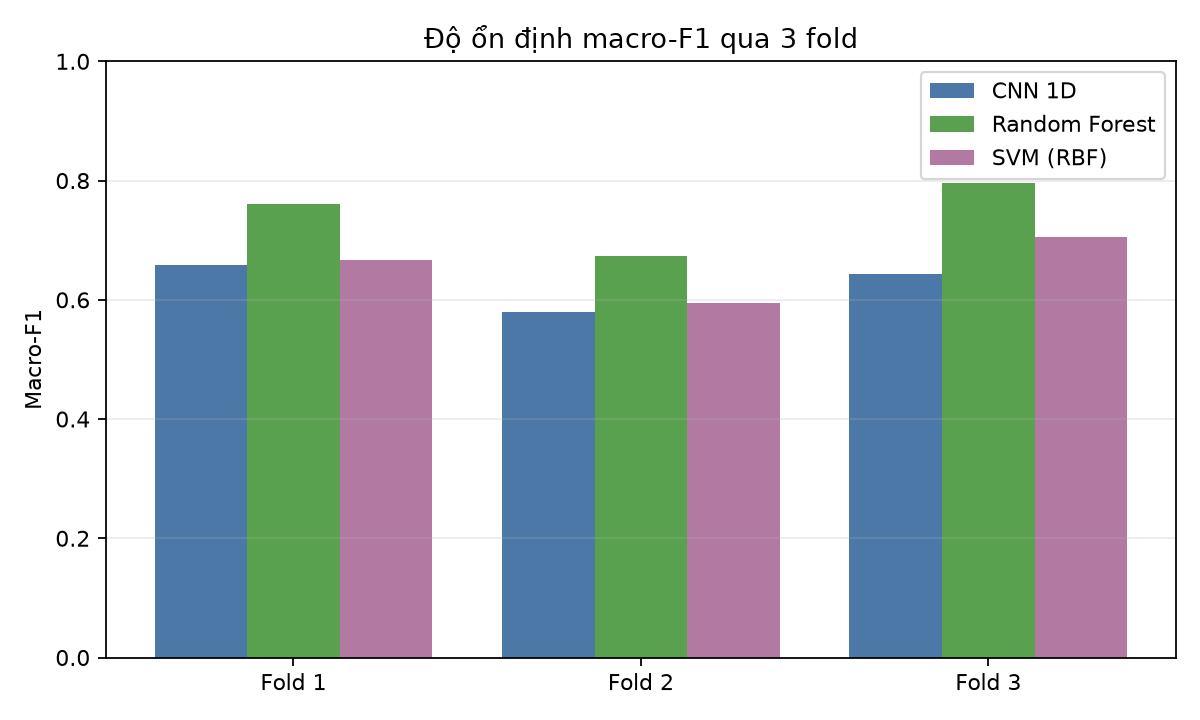
\includegraphics[width=0.78\textwidth]{figures/simple_fold_macro_f1.png}
    \caption{Macro-F1 của từng mô hình qua 3 fold}
    \label{fig:fold-f1}
\end{figure}

Bảng \ref{tab:fold-results} và Hình \ref{fig:fold-f1} thể hiện hiệu năng của các mô hình qua từng fold đánh giá. Random Forest cho thấy sự ổn định tốt nhất, mặc dù điểm Macro-F1 ở Fold 2 giảm xuống còn 0.6732 so với hai fold còn lại (đều trên 0.76). Cả ba mô hình đều đạt kết quả thấp nhất ở Fold 2 (CNN giảm xuống 0.5804, SVM xuống 0.5944), điều này chỉ ra rằng tập dữ liệu ở Fold 2 có thể chứa nhiều biến động hành vi phức tạp hơn hoặc có sự khác biệt lớn về phân phối dữ liệu giữa tập huấn luyện và kiểm định so với các fold khác.

\subsection{Accuracy của Random Forest}

\begin{figure}[H]
    \centering
    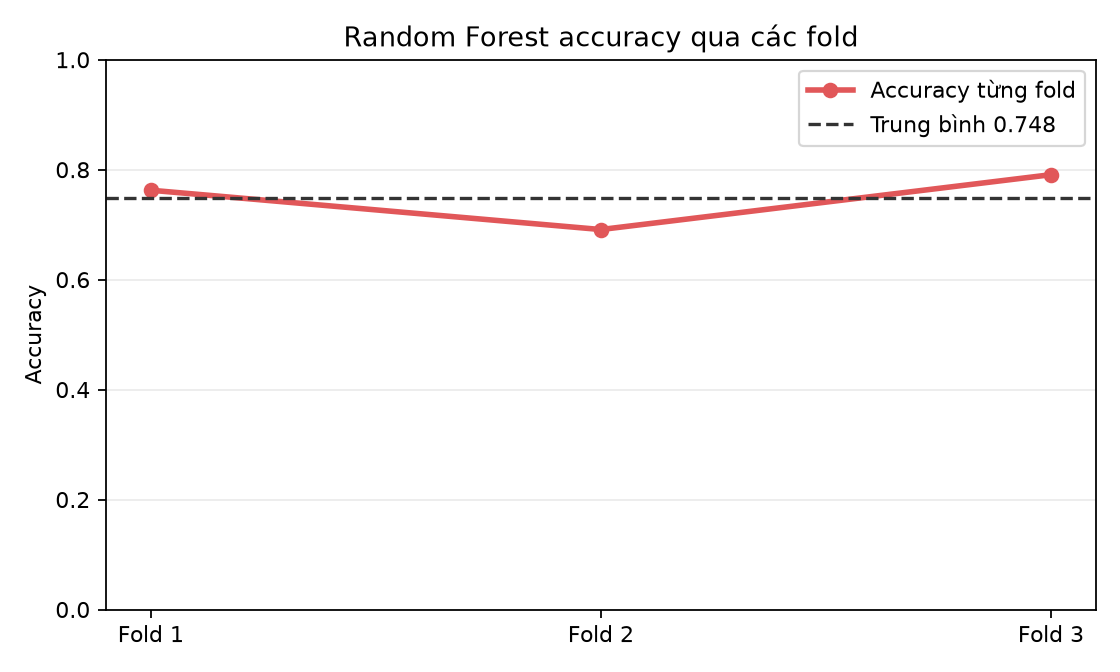
\includegraphics[width=0.78\textwidth]{figures/simple_rf_accuracy.png}
    \caption{Accuracy của Random Forest qua từng fold}
    \label{fig:rf-accuracy}
\end{figure}

Accuracy trung bình của Random Forest đạt 0.7482, cao hơn macro-F1 (0.7434) một khoảng nhỏ. Chênh lệch này cho thấy mô hình dự đoán các người dùng có nhiều cửa sổ tốt hơn so với các người dùng ít dữ liệu; macro-F1 vì vậy phản ánh sát hơn hiệu năng trên toàn bộ 15 lớp khi dữ liệu không cân bằng.

\subsection{Phân tích mô hình Random Forest}

Để hiểu mô hình chính dựa vào tín hiệu nào, Hình \ref{fig:rf-importance} liệt kê 20 đặc trưng có mức độ quan trọng (Gini importance) cao nhất do Random Forest tính ra. Các đặc trưng dẫn đầu chủ yếu thuộc nhóm thống kê biên độ và năng lượng của các trục gia tốc và con quay, cho thấy đặc trưng phân biệt người dùng nằm phần lớn ở mức độ và cường độ chuyển động, hơn là ở các đặc trưng tần số.

\begin{figure}[H]
    \centering
    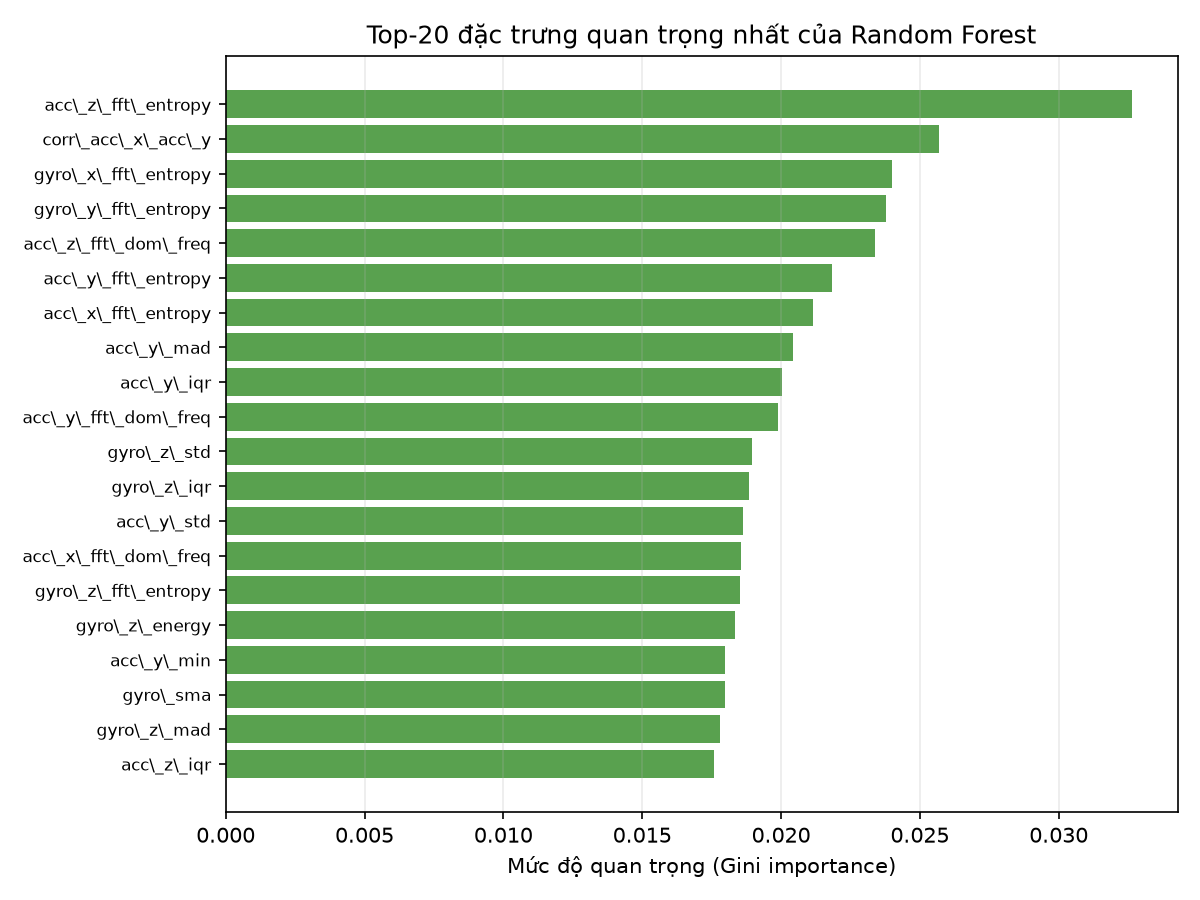
\includegraphics[width=0.85\textwidth]{figures/rf_feature_importance.png}
    \caption{Top-20 đặc trưng quan trọng nhất theo Gini importance của Random Forest}
    \label{fig:rf-importance}
\end{figure}

Hình \ref{fig:pca} chiếu 65 đặc trưng xuống 2 thành phần chính (PCA), tô màu theo người dùng. Một số người dùng tạo thành cụm tách biệt, nhưng nhiều cụm chồng lấn nhau, phản ánh trực quan vì sao bài toán không đạt độ chính xác tuyệt đối: trong không gian đặc trưng, hành vi của một số người dùng tương đối giống nhau. PCA chỉ giữ hai chiều phương sai lớn nhất nên mức chồng lấn thực tế mà mô hình xử lý trong không gian 65 chiều thấp hơn hình minh hoạ.

\begin{figure}[H]
    \centering
    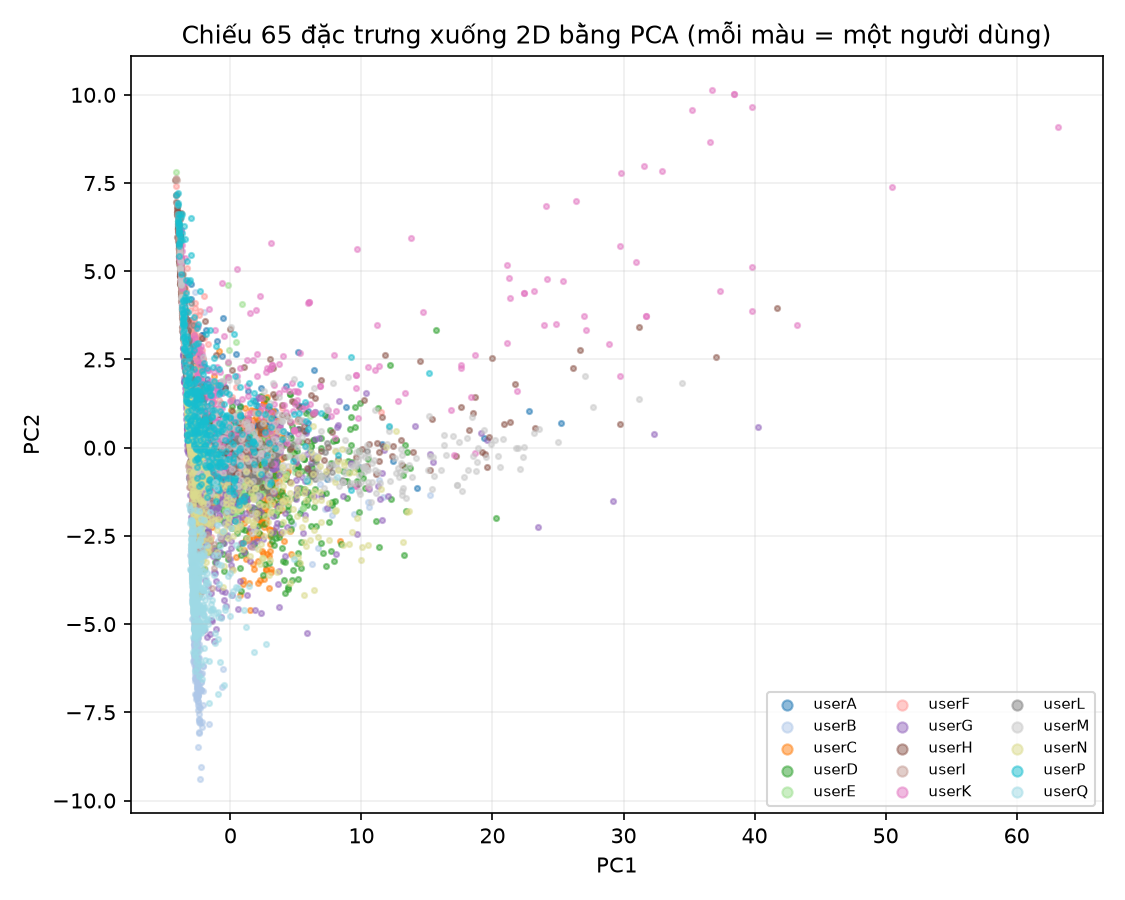
\includegraphics[width=0.85\textwidth]{figures/feature_pca.png}
    \caption{Phân bố các cửa sổ trong không gian 2 thành phần chính (PCA) của 65 đặc trưng, tô màu theo người dùng}
    \label{fig:pca}
\end{figure}

Hình \ref{fig:rf-confusion} là ma trận nhầm lẫn chuẩn hoá theo hàng của Random Forest, gom dự đoán out-of-fold trên cả 3 fold. Đường chéo đậm cho thấy phần lớn cửa sổ được phân đúng người dùng; các ô lệch khỏi đường chéo chỉ ra những cặp người dùng dễ bị nhầm với nhau, thường là các cặp có biên độ chuyển động tương tự.

\begin{figure}[H]
    \centering
    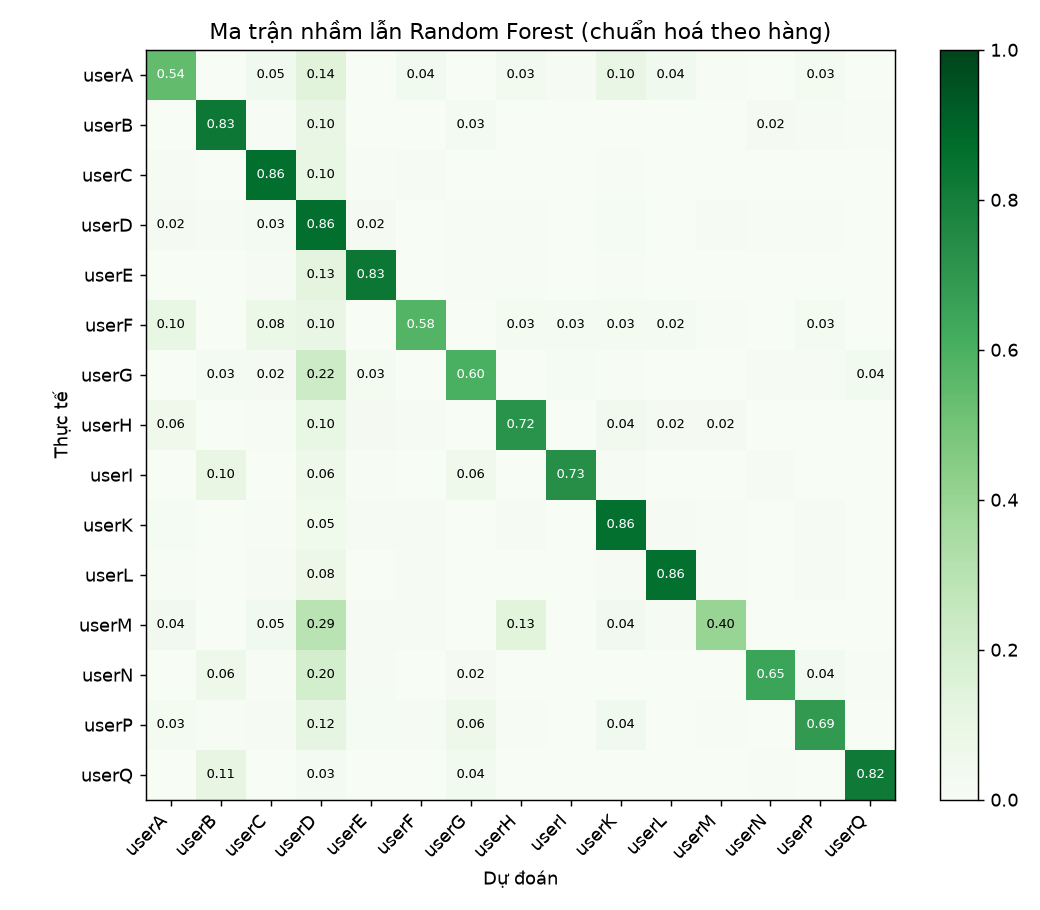
\includegraphics[width=0.82\textwidth]{figures/rf_confusion.png}
    \caption{Ma trận nhầm lẫn chuẩn hoá của Random Forest trên 15 người dùng (gom 3 fold)}
    \label{fig:rf-confusion}
\end{figure}

\subsection{Phân tích CNN theo hoạt động}

Pipeline đánh giá tổng hợp (\texttt{python -m src.evaluate}) còn sinh biểu đồ hiệu năng theo hoạt động và ma trận nhầm lẫn cho CNN. Hai hình này dùng để phân tích sâu hơn các lỗi của mô hình CNN trên 15 người dùng.

\begin{figure}[H]
    \centering
    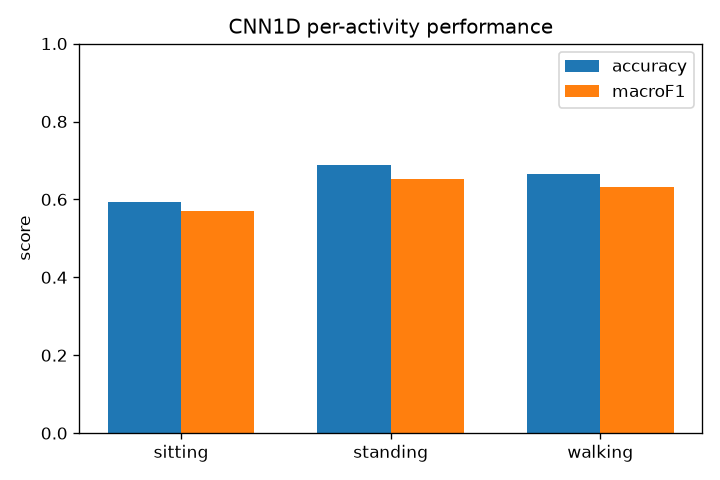
\includegraphics[width=0.72\textwidth]{figures/cnn_per_activity.png}
    \caption{Hiệu năng CNN theo hoạt động sitting, standing, walking}
    \label{fig:per-activity}
\end{figure}

\begin{figure}[H]
    \centering
    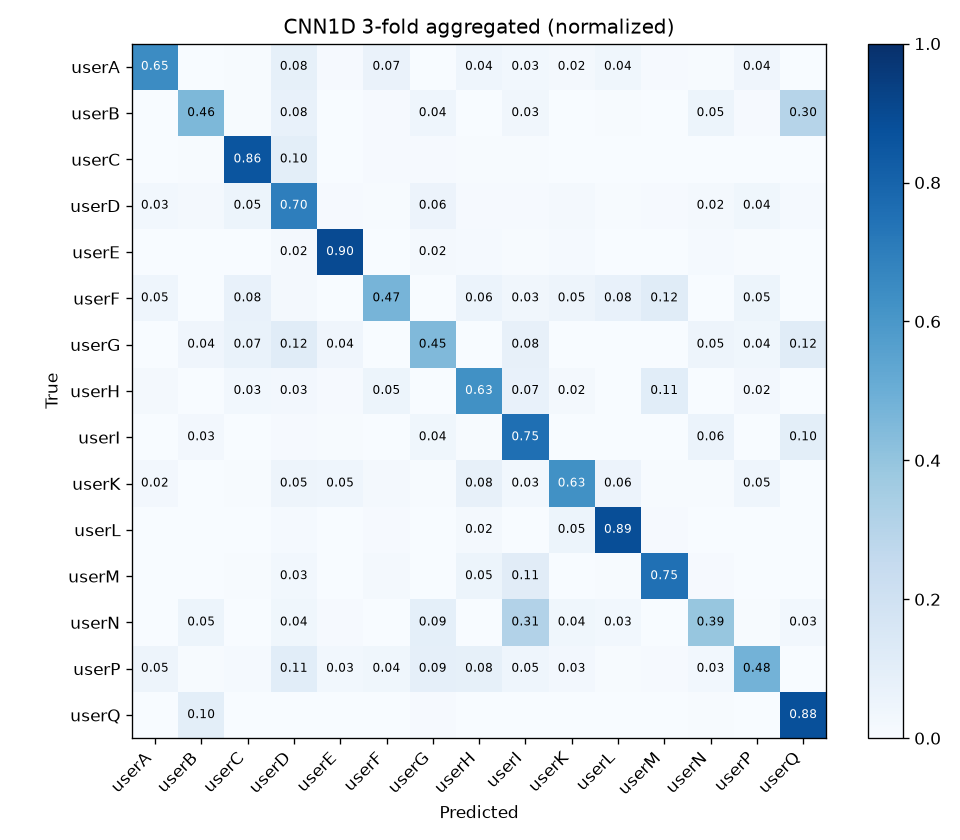
\includegraphics[width=0.82\textwidth]{figures/cnn_confusion.png}
    \caption{Ma trận nhầm lẫn chuẩn hoá của CNN}
    \label{fig:confusion}
\end{figure}

\section{Các chức năng chính của hệ thống và cách sử dụng}

\subsection{Chức năng chính}

Hệ thống được tổ chức thành các bước độc lập, có thể chạy lại từng phần.

\begin{longtable}{P{0.08\textwidth}P{0.37\textwidth}P{0.39\textwidth}}
\caption{Các chức năng chính của hệ thống} \\
\toprule
STT & Lệnh & Chức năng \\
\midrule
\endfirsthead
\toprule
STT & Lệnh & Chức năng \\
\midrule
\endhead
1 & \path{python -m src.io} & Quét dữ liệu thô, parse tên file, sinh \texttt{manifest.csv}. \\
2 & \path{python -m src.preprocess} & Tiền xử lý cảm biến, lọc tín hiệu, chia cửa sổ, sinh \texttt{windows.npz}. \\
3 & \path{python -m src.features} & Trích đặc trưng gõ phím phục vụ phân tích bổ sung. \\
4 & \path{python -m scripts.run_simple_pipeline} & Chạy pipeline đơn giản gồm CNN 1D, RF và SVM, lưu \texttt{simple\_results.json}. \\
5 & \path{python -m src.evaluate} & Gom prediction CNN, vẽ ma trận nhầm lẫn và per-activity, chạy RF/SVM, lưu \texttt{evaluate\_results.json}. \\
6 & \path{python -m scripts.plot_simple_results} & Vẽ biểu đồ so sánh mô hình, fold và accuracy. \\
7 & \path{jupyter lab simple_pipeline.ipynb} & Chạy notebook minh hoạ kết quả và biểu đồ trong JupyterLab. \\
\bottomrule
\end{longtable}

\subsection{Cài đặt môi trường}

Yêu cầu Python 3.10 trở lên. Các gói chính được liệt kê trong \texttt{requirements.txt}: \texttt{numpy}, \texttt{pandas}, \texttt{scipy}, \texttt{scikit-learn}, \texttt{torch}, \texttt{matplotlib}, \texttt{seaborn}, \texttt{joblib}, \texttt{tqdm}, \texttt{jupyterlab}.

\begin{lstlisting}[language=bash]
python3 -m venv venv
source venv/bin/activate
pip install -r requirements.txt --index-url https://pypi.org/simple
\end{lstlisting}

\subsection{Chạy pipeline đơn giản}

\begin{lstlisting}[language=bash]
source venv/bin/activate
python -m scripts.run_simple_pipeline
python -m scripts.plot_simple_results
\end{lstlisting}

Kết quả chính:

\begin{itemize}
    \item \texttt{simple\_results.json}: điểm số CNN và RF.
    \item \texttt{simple\_model\_comparison.png}: so sánh tổng thể.
    \item \texttt{simple\_fold\_macro\_f1.png}: điểm từng fold.
    \item \texttt{simple\_rf\_accuracy.png}: accuracy của RF.
\end{itemize}

\subsection{Chạy bằng JupyterLab}

Nhóm đã chuẩn bị notebook \texttt{simple\_pipeline.ipynb}. Mở notebook bằng:

\begin{lstlisting}[language=bash]
source venv/bin/activate
jupyter lab simple_pipeline.ipynb
\end{lstlisting}

Trong notebook, biến \texttt{RUN\_TRAIN} mặc định là \texttt{False} để không train lại CNN mỗi lần mở. Nếu muốn chạy lại toàn bộ, đổi \texttt{RUN\_TRAIN = True}. Nếu chỉ muốn cập nhật RF và biểu đồ, đổi \texttt{RUN\_RF\_ONLY = True}.

\section{Cấu trúc mã nguồn và vai trò các class/method chính}

\subsection{Tổ chức mã nguồn}

Mã nguồn được tách theo đúng luồng xử lý: đọc dữ liệu, tiền xử lý, định nghĩa dataset, huấn luyện, đánh giá và vẽ hình. Trong báo cáo chỉ nêu tên file chính để tránh làm phần trình bày bị nặng bởi đường dẫn thư mục.

\subsection{Vai trò các module chính}

\begin{longtable}{P{0.34\textwidth}P{0.56\textwidth}}
\caption{Vai trò các module chính} \\
\toprule
File & Vai trò \\
\midrule
\endfirsthead
\toprule
File & Vai trò \\
\midrule
\endhead
\texttt{config.py} & Khai báo đường dẫn, kích thước cửa sổ, danh sách kênh cảm biến, danh sách hoạt động, seed. \\
\texttt{io.py} & Parse tên file, đọc CSV, ước lượng tần số lấy mẫu, xây dựng manifest. \\
\texttt{preprocess.py} & Resample, lọc Butterworth, tách trọng lực, chia sliding window. \\
\texttt{features.py} & Trích đặc trưng thống kê, FFT, correlation, SMA và đặc trưng keystroke. \\
\texttt{datasets.py} & Định nghĩa \texttt{InertialDataset}, chuẩn hoá dữ liệu, chuyển shape cho Conv1D. \\
\texttt{models.py} & Định nghĩa \texttt{CNN1D} và factory \texttt{make\_model}. \\
\texttt{train.py} & Chạy huấn luyện 3-fold, lưu checkpoint và log experiment. \\
\texttt{evaluate.py} & Chạy Random Forest và SVM (RBF) baseline, gom prediction CNN, vẽ confusion/per-activity. \\
\texttt{run\_simple\_pipeline.py} & Script đơn giản hoá để chạy ba mô hình chính: CNN 1D, RF và SVM. \\
\texttt{plot\_simple\_results.py} & Tạo các biểu đồ chính dùng trong báo cáo. \\
\bottomrule
\end{longtable}

\subsection{Class và method quan trọng}

\begin{itemize}
    \item \texttt{InertialDataset.\_\_getitem\_\_}: lấy một cửa sổ cảm biến, chuẩn hoá theo mean/std của train fold, chuyển từ shape \((T, C)\) sang \((C, T)\) cho PyTorch Conv1D.
    \item \texttt{CNN1D.forward}: chạy chuỗi Conv1D, BatchNorm, ReLU, pooling và linear head để dự đoán người dùng.
    \item \texttt{run\_cv}: thực hiện vòng lặp 3-fold, gọi train từng fold, lưu checkpoint và metric.
    \item \texttt{rf\_baseline}: trích đặc trưng thủ công, chuẩn hoá, train Random Forest và tính macro-F1/accuracy.
    \item \texttt{svm\_baseline}: dùng cùng 65 đặc trưng và quy trình chuẩn hoá như \texttt{rf\_baseline}, train SVM RBF và tính macro-F1/accuracy.
    \item \texttt{plot\_model\_comparison}, \texttt{plot\_fold\_scores}, \texttt{plot\_rf\_accuracy}: sinh hình minh hoạ kết quả.
\end{itemize}

\section{Khó khăn gặp phải và cách giải quyết}

\subsection{Tên file và schema dữ liệu không đồng nhất}

Các file dữ liệu có nhiều quy ước đặt tên khác nhau, ví dụ \texttt{\_s1\_att2.csv}, \texttt{\_s1\_r3.csv}, hoặc thiếu một số thành phần. Nếu parse thủ công từng trường hợp, pipeline dễ lỗi và khó mở rộng. Nhóm xử lý bằng các regex riêng trong \texttt{io.py}, sau đó sinh manifest thống nhất.

\subsection{Nguy cơ rò rỉ dữ liệu khi chia train/validation}

Nếu chia ngẫu nhiên theo cửa sổ, các cửa sổ từ cùng một file có thể xuất hiện ở cả train và validation. Do cửa sổ trượt có overlap 50\%, nhiều mẫu liền kề gần như cùng biểu diễn một đoạn chuyển động. Điều này làm điểm số tăng giả tạo vì mô hình học đặc trưng riêng của phiên ghi thay vì học hành vi người dùng. Giải pháp là dùng \textit{StratifiedGroupKFold} theo group \texttt{user\_\_file}, đảm bảo cùng một file không bị tách sang hai tập.

\subsection{Ít file ở một số người dùng}

Số file inertial giữa các user không đều. User ít nhất là \texttt{userQ}, chỉ có 3 file inertial. Nếu cố dùng 5-fold, một số fold validation có thể thiếu user này, làm macro-F1 không đánh giá đủ class và khiến kết quả kém tin cậy. Giải pháp là chọn 3-fold, cân bằng giữa số lần đánh giá và điều kiện mỗi fold vẫn có đủ 15 người dùng.

\subsection{Mất cân bằng số cửa sổ giữa các file}

Một số file dài sinh ra rất nhiều cửa sổ, khiến một vài người dùng hoặc phiên ghi chi phối dữ liệu huấn luyện. Giải pháp là giới hạn tối đa 300 cửa sổ mỗi file và lấy mẫu đều theo thời gian bằng \texttt{np.linspace}.

\subsection{Dữ liệu cảm biến có nhiễu và khác tần số}

Dữ liệu thực tế từ điện thoại có thể lệch tần số lấy mẫu hoặc nhiễu cao tần. Pipeline xử lý bằng cách resample về 50 Hz, low-pass 20 Hz và high-pass 0.3 Hz cho gia tốc.

\subsection{CNN không vượt Random Forest}

Kết quả cho thấy Random Forest đạt macro-F1 0.7434, cao hơn CNN 1D (0.6272) khoảng 0.116. Với tập 39018 cửa sổ và số phiên ghi giới hạn cho mỗi người dùng, CNN chưa đủ dữ liệu để học biểu diễn vượt qua bộ 65 đặc trưng thống kê đã mã hoá sẵn thông tin về biên độ, năng lượng, tần số và tương quan giữa các trục. Đây là hiện tượng thường gặp khi áp dụng học sâu trên tập dữ liệu cỡ vừa và nhỏ.

\section{Khám phá mới hoặc kết luận}

\subsection{Khám phá chính}

\begin{enumerate}
    \item \textbf{Random Forest đạt hiệu năng cao nhất trong ba mô hình}. Với macro-F1 0.7434, Random Forest vượt SVM RBF (0.6550) và CNN 1D (0.6272) trên cùng điều kiện đánh giá, nên được chọn làm mô hình chính của báo cáo.
    \item \textbf{Đánh giá group-by-file là bắt buộc}. Nếu không nhóm theo file, kết quả có thể bị leakage và không phản ánh khả năng tổng quát hoá tới phiên ghi mới.
    \item \textbf{Hai mô hình trên cùng đặc trưng cho kết quả gần nhau}. Random Forest và SVM RBF dùng chung 65 đặc trưng và cho điểm tương đồng, cho thấy phần lớn hiệu năng đến từ chất lượng đặc trưng thủ công chứ không phải từ một loại mô hình cụ thể.
    \item \textbf{Dữ liệu chuyển động giàu thông tin hơn khi hoạt động có chuyển động rõ}. Các hoạt động như walking/standing thường cho tín hiệu phân biệt người dùng tốt hơn sitting.
    \item \textbf{Deep learning không phải lúc nào cũng thắng}. Trong bối cảnh dữ liệu nhỏ, mô hình cổ điển với feature tốt có thể vượt mô hình CNN đơn giản.
\end{enumerate}

\subsection{Kết luận}

Đồ án đã hoàn thành pipeline từ dữ liệu thô tới đánh giá mô hình: đọc CSV, chuẩn hoá manifest, tiền xử lý cảm biến, chia cửa sổ, trích đặc trưng, huấn luyện ba mô hình (Random Forest, SVM RBF, CNN 1D), đánh giá closed-set 15 người dùng và sinh biểu đồ báo cáo.

\begin{itemize}
    \item Random Forest: mô hình chính, đạt macro-F1 0.7434 và accuracy 0.7482.
    \item SVM (RBF): baseline thứ hai trên cùng đặc trưng, đạt macro-F1 0.6550.
    \item CNN 1D: mô hình học sâu bổ sung, đạt macro-F1 0.6272.
\end{itemize}

\subsection{Hướng phát triển}

\begin{itemize}
    \item Thu thêm dữ liệu nhiều phiên hơn cho mỗi người dùng.
    \item Kết hợp inertial với keystroke ở mức feature fusion.
    \item Thử thêm đặc trưng hoặc tinh chỉnh siêu tham số cho CNN để rút ngắn khoảng cách với mô hình cổ điển.
    \item Tạo giao diện demo đơn giản để upload CSV và dự đoán người dùng.
\end{itemize}

\subsection{Đóng gói sản phẩm nộp}

\begin{itemize}
    \item Mã nguồn dự án và cấu hình thí nghiệm.
    \item Hướng dẫn cài đặt và chạy: \texttt{README.md} và \texttt{requirements.txt}.
    \item Báo cáo cuối: \texttt{bao\_cao.pdf}.
    \item Notebook minh hoạ: \texttt{simple\_pipeline.ipynb}.
    \item Kết quả số: \texttt{simple\_results.json}.
    \item Các hình kết quả dùng trong báo cáo.
\end{itemize}


\begin{thebibliography}{9}
\bibitem{sklearn}
Pedregosa et al., \textit{Scikit-learn: Machine Learning in Python}, Journal of Machine Learning Research, 2011.

\bibitem{pytorch}
Paszke et al., \textit{PyTorch: An Imperative Style, High-Performance Deep Learning Library}, NeurIPS, 2019.

\bibitem{scipy}
Virtanen et al., \textit{SciPy 1.0: Fundamental Algorithms for Scientific Computing in Python}, Nature Methods, 2020.

\bibitem{uci-har}
Anguita et al., \textit{A Public Domain Dataset for Human Activity Recognition Using Smartphones}, ESANN, 2013.
\end{thebibliography}

\end{document}
